\subsection{Determinant of Hessian}
Determinant of Hessian $DoH$ udgør feature detektoren i SURF. $DoH$ er baseret på Hessian matricen, som udregnes for hvert punkt $p$ i et billede:
\begin{equation}
\mathcal{H}(p, \sigma) = 
 \begin{bmatrix}
 	L_{xx}(p, \sigma) & L_{xy}(p, \sigma) \\
 	L_{xy}(p, \sigma) & L_{yy}(p, \sigma) 
 \end{bmatrix}
 \label{hessianmatrix}
\end{equation}
hvor $\sigma$ angiver skala og $L_{xx}$ defineres som: 
\begin{equation}
L_{xx}(x, \sigma) = (\frac{\partial^2 }{\partial x^2 } G(x,y,\sigma)) * I
\label{lxx}
\end{equation}
og analogt for $L_{yy}, L_{xy}$. Bay et al. anvender approkismerede boksfiltre: $D_{xx}$, $D_{yy}$ og $D_{xy}$, der udelukkende består af værdierne $-2,-1,0, 1$ som ved brug af integralbilleder nedsætter antallet af beregninger drastisk. I denne implementering er disse boksfiltre ikke anvendt, men udregnet som ligning \eqref{lxx}. Figur \ref{fig:lxxlyylxy} er en illustration af de afledte Gaussiske filtre, der er anvendt. Denne designbeslutning skyldes, at beregningerne af integralbilleder komplicerede programmet. Da 
boksfiltrene er en approksimation til $L$ er denne tilgang korrekt.
\begin{figure}[H]
    \centering
    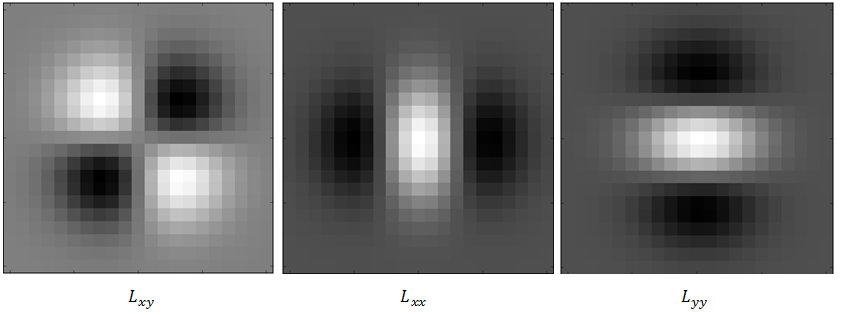
\includegraphics[width=0.75\textwidth]{fig/31.png}
     \vspace{-0.5em}
    \begin{center}    
       \caption{\textcolor{gray}{\footnotesize \textit{ }}}
    \label{fig:lxxlyylxy}
     \end{center}
     \vspace{-2.5em}
  \end{figure} \noindent
I SURF oprettes et skalarum, der ligesom i SIFT opdeles i skalaer og oktaver. I stedet for at reducere billedernes størrelser, forøges størrelserne af de anvendte filtre. SIFT anvender en stigende sigma værdi, med en fast filterstørrelse. For hver oktav anvendes der, i denne implementering, fire billeder foldet med fire forskellige filterstørrelser. For hver oktav bruges nr. 2 filterstørrelse, fra forrige oktav til startoktav (startende på størelse 9), og størrelsen imellem filtre, fordobles fra forrige oktav, som vist i tabel \ref{fig:secderivfiltersize}. Her skal det bemærkes, at de andenafledte filtre, skal have dobbelt størrelse, af de førsteafledte.
\begin{figure}[H]
    \centering
    \begin{center}    
    \begin{tabular}{ | l | l | l | l | l |}
    \hline
    oktav & filter str 1 & filter str 2 & filter str 3 & filter str 4 \\ \hline
    1 & 9 & 15 & 21 & 27 \\ \hline
  	2 & 15 & 27 & 39 & 51 \\ \hline
  	3 & 27 & 51 & 75 & 99 \\ \hline
  	4 & 51 & 99 & 147 & 195 \\ \hline
    \end{tabular}       
    \caption{\textcolor{gray}{\footnotesize \textit{Fire forskellige oktaver, og filterstørrelse, for et andenafledt filter}}}
    \label{fig:secderivfiltersize}
     \end{center}
     \vspace{-2.5em}
  \end{figure} \noindent
For hvert punkt i billederne opstilles Hessian matricen, hvorefter determinanten udregnes for alle punkter i billederne. Bay et.al. udregner determinanten ved:
\begin{equation}
\textbf{det}\mathcal{H}_{approksimeret} = D_{xx}D_{yy}-wD_{xy}^2
\label{deerminantofhessian}
\end{equation}
hvor $w$ er en vægt, tilføjet for at balancere de approksimerede differentierede Gaussiske filtre og boksfiltrene. Da denne implementering ikke anvender boksfiltre, udregnes determinanten som:
\begin{equation}
\textbf{det}\mathcal{H} = L_{xx}L_{yy}-L_{xy}^2
\label{deerminantofhessian}
\end{equation}
Blobs er lokaliseret på lokale ekstremaer. Når hessian matricens egenværdier har samme fortegn, indikere dette et ekstrema:
\begin{equation}
\begin{split}
\text{indikator} = 
\begin{cases}
\text{Ekstrema}& \text{hvis } \bold{det}(\mathcal{H}) > 0,  \\
\text{Saddel-Punkt} & \text{hvis } \bold{det}(\mathcal{H}) < 0.
\end{cases}
\end{split}
\label{detman}
\end{equation}
Et punkt udvælges, hvis det er det største af et $3\times3\times3$ område af determinant billederne, som vist i figur \ref{fig:difference}. Dette udføres for alle oktaver. Non-maximal surpression anvendes ligesom i SIFT.
\\
\\
\subsubsection*{Algoritme: SURF interessepunkts detektor}
\begin{enumerate}
\item[Input:] Billede $I$
\item[Output:] Interessepunkter $p \in (x,y)$
\end{enumerate}
\begin{enumerate}
\item {Hessian matricen opstilles for alle punkter i skalabillederne som i ligning \eqref{hessianmatrix}}
\item Determinantbilleder opstilles, ved at udregne determinanten af Hessian matricen for alle punkter i alle billeder som i ligning \eqref{deerminantofhessian}.
\item Lokale maxima udvælges, af hvert $3\times3\times3$ område af billeder på samme oktav.
\item Accurate keypoint localisation, bruges til at fjerne dårligt lokaliserede punkter ligesom i ligning \eqref{maxsurp}.
\end{enumerate}